\chapter{Implementation and Experimental Results}
\label{ch:implementation}

Thus far, we have only discussed our system from a theoretical perspective.
Henceforth, we evaluate out system experimentally and compare the results with the theoretical analysis.
We begin this chapter by a description of the implementation in \Cref{sec:implementation}.
Then, we move on to describing our experimental setup in \Cref{sec:experimental-setup}.
Finally, \Cref{sec:evaluation} presents our experimental results and our evaluation.
Our experiment primarily focuses on the consensus duration and the throughput.


\section{Implementation}
\label{sec:implementation}

The prototype implementation is done in the event driven paradigm, using the Python programming language.
We use Twisted as our networking library.
The code can be found on GitHub\footnote{\url{https://github.com/kc1212/consensus-thesis-code}}.

The structure of the implementation is primarily made up of three modules---\texttt{acs}, \texttt{trustchain} and \texttt{node}.
\texttt{acs}, as its name suggests, implements ACS.
We use liberasurecode\footnote{\url{https://github.com/openstack/liberasurecode}} as the Reed-Solomon error correcting code library, used in RBC.
An implementation detail is that liberasurecode cannot create more than 32 code blocks\footnote{
  The 32 code blocks limitation is hardcoded in the source file, see
  \url{https://github.com/openstack/liberasurecode/blob/0794b31c623e4cede76d66be730719d24debcca9/include/erasurecode/erasurecode.h\#L35}
}.
The \texttt{acs} module provides a small interface to the caller to start and stop the consensus process and also receive results.
The \texttt{trustchain} module implements the Extended TrustChain data structure.
It also provides the essential algorithm necessary to interact with Extended TrustChain such as 
$\textsf{new\_tx}(\cdot)$, $\textsf{new\_cp}(\cdot)$, $\textsf{agreed\_fragment}(\cdot)$ and so on.
Since this is a prototype implementation, we only store the data structure in memory and not on disk.
Finally, the \texttt{node} module ties everything together.
It implements the the consensus phase, the transaction protocol and the validation protocol.

Every node keeps a persistent TCP connection with every other node.
This creates a fully connected network for our experiment.
It is certainly not idea in real world scenarios where nodes may have limited resources.
But as a prototype, it is sufficient to create a system that has just over a thousand nodes, which is enough for us to experiment on.

\section{Experimental Setup}
\label{sec:experimental-setup}

There are two asppects of the experimental setup.
First is the nature of the experiment.
Second is the physical setup.
We describe these in turn.

The nature and the goal of the experiment is to run the three protocols---consensus protocol,
transaction protocol and validation protocol---simultaneously and analyse the throughput and consensus duration.
There are two types of parameters which we must consider.
First are the fixed parameters $r_{\text{tx}}$ and $D$.
These are selected from emperical evidence, we found that $D = 30$ seconds to be more than enough for all CP blocks to reach consensus.
We also found that using $r_{\text{tx}} = 8$ gave us good throughput without putting too much demand on the bandwidth which is must also be used for ACS.
These parameters are fixed for all our experiments.
The second set of parameters can be seen as the domain,
and we run our experiment for every combination of these parameters.
Concretely, there are three of them.
The number of facilitators $n \ in \{ 8, 12, \dots, 32\}$.
The population size $N \in \{100, 200, \dots, 1200\}$.
Finally the two modes of transaction.
The first mode or the ideal mode is that nodes only transact with their immediate neighbour. 
This minimises the bandwidth required per validated transaction because agreed fragment can be cached.
The second mode is in the other extreme, where  every transaction is with a random node out of the $N$ nodes in the system,
thus the agreed fragment is unlikely to be cached.
Unfortunately, the maximum $n$ is 32 because the limitation in liberasurecode mentioned in \Cref{sec:implementation}.
$N$ stops at 1200 is due to our physical setup, which we describe next.

The experiment is run on the DAS-5 (The Distributed ASCI Supercomputer 5).
From now on, we use "machines" to refer to DAS-5 nodes and nodes to refer to a running instance in our system.
On DAS-5 we use up to 24 machine, for each machine we use 50 nodes.
This gives us the aforementioned 1200 number.
With this setup, we cannot run more nodes because the every machine only has 65535 ports available (some of them are reserved).
But 50 nodes each need 1200 TCP connections which is 60000 TCP connections per machine.
Thus we set $N$ to be at most 1200\footnote{While it is possible to have many more TCP connections per machine,
but it requires additional network interface which is something we do not control on the DAS-5.}.
% TODO contradicts with the fully connected argument before

To coordinate nodes on many different machine,
we employ a discovery server to inform every node the IP addresses and port numbers of every other node.
It is only run before the experiment and is not used during the experiment.


\section{Evaluation}
\label{sec:evaluation}

\subsection{Consensus Duration}

\begin{figure}[h]
  \centering
  \begin{subfigure}{\textwidth}
    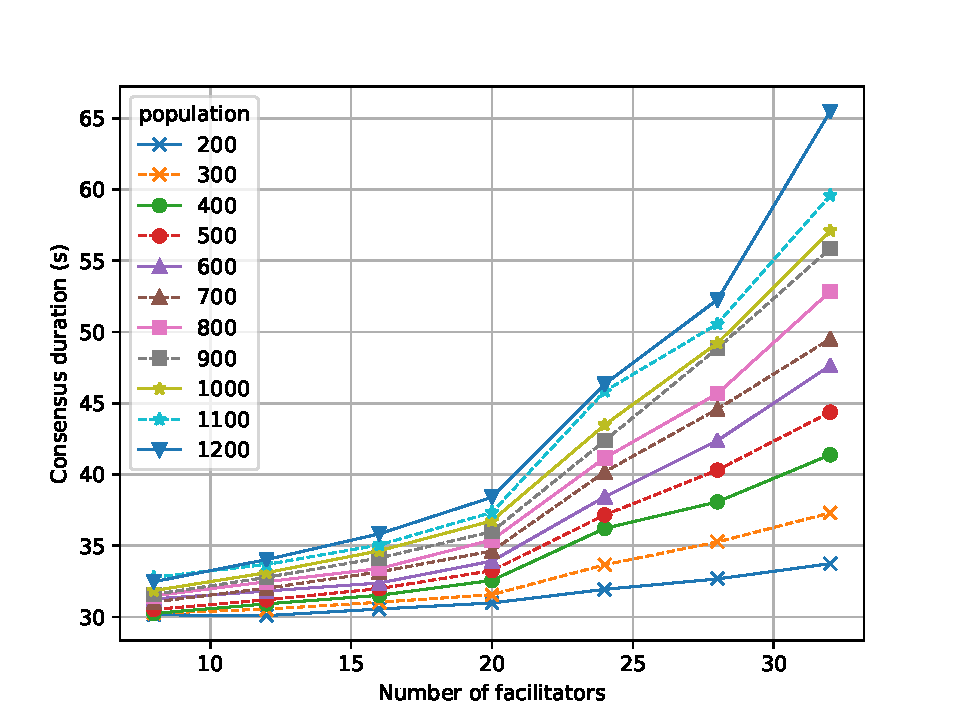
\includegraphics[width=\textwidth]{result-normal-cons-vs-facilitator}
  \end{subfigure}

  \begin{subfigure}{\textwidth}
    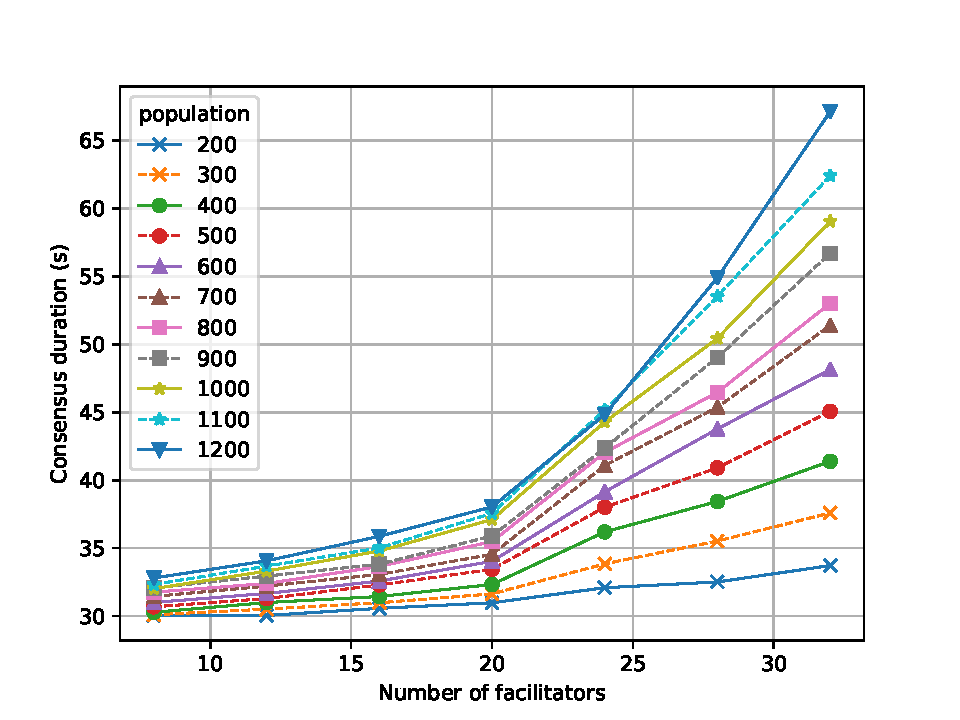
\includegraphics[width=\textwidth]{result-rand-cons-vs-facilitator}
  \end{subfigure}
\end{figure}

\begin{figure}[h]
  \centering
  \begin{subfigure}{\textwidth}
    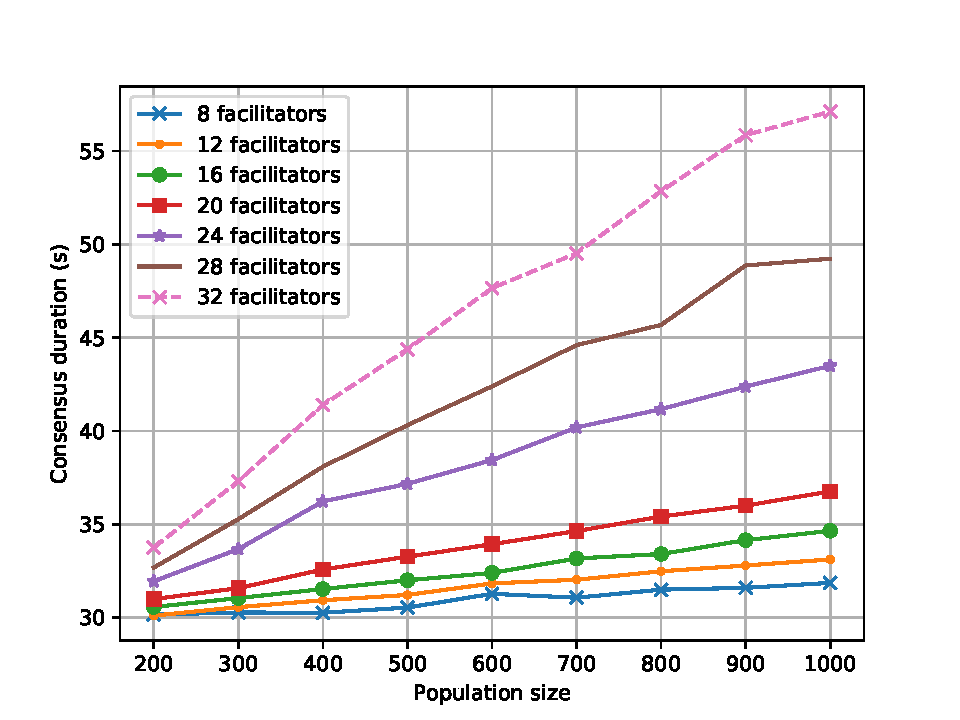
\includegraphics[width=\textwidth]{result-normal-cons-vs-pop}
  \end{subfigure}

  \begin{subfigure}{\textwidth}
    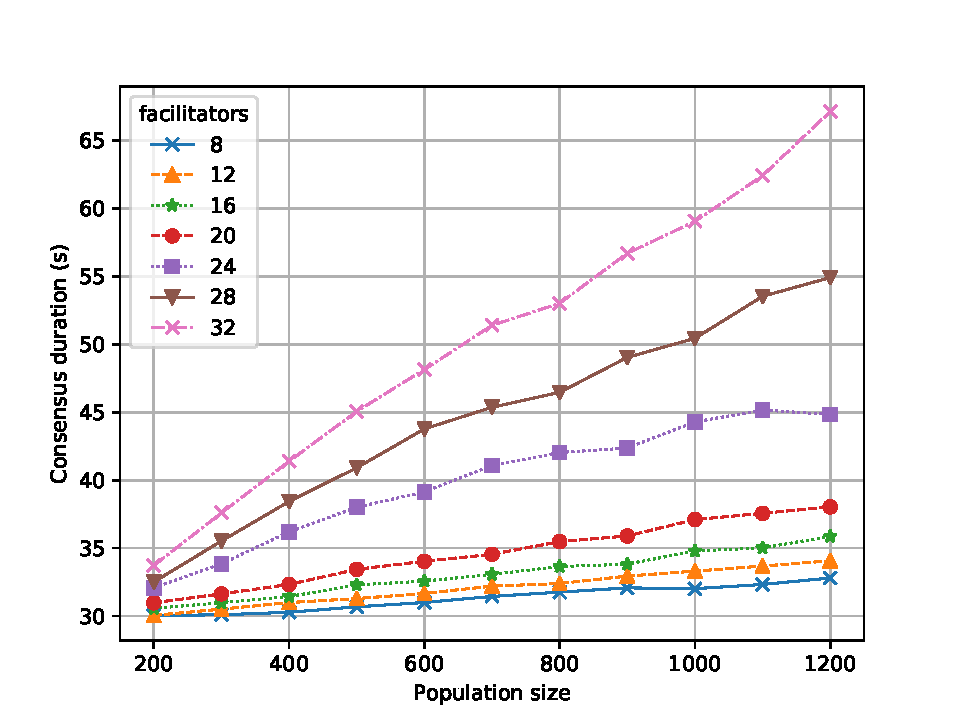
\includegraphics[width=\textwidth]{result-rand-cons-vs-pop}
  \end{subfigure}
\end{figure}

\subsection{Global Throughput}

\begin{figure}[h]
  \centering
  \begin{subfigure}{\textwidth}
    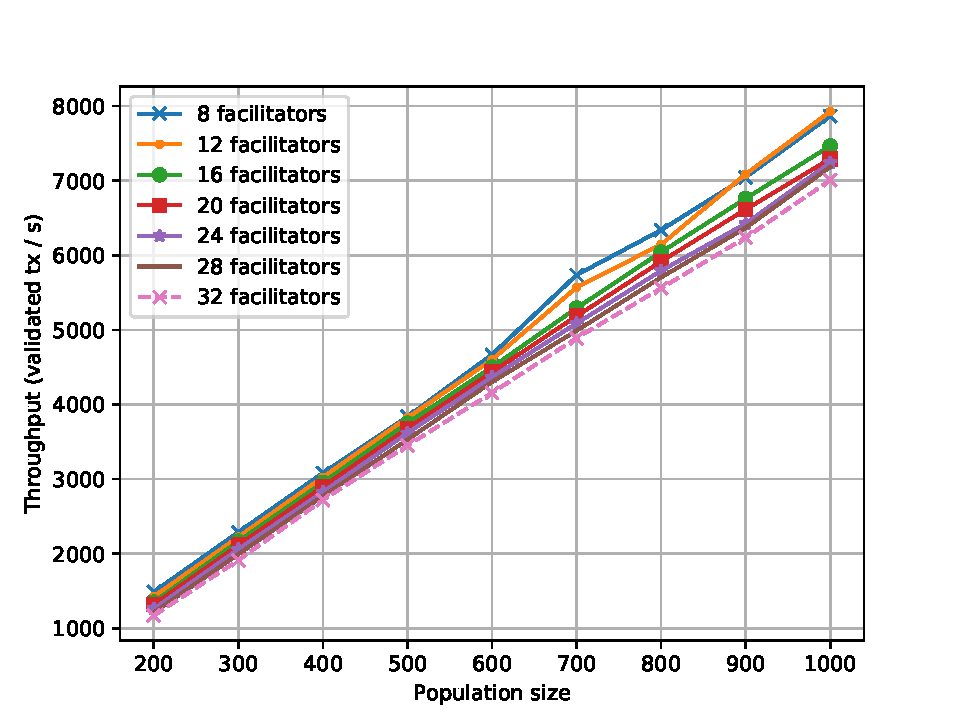
\includegraphics[width=\textwidth]{result-normal-throughput-vs-pop}
  \end{subfigure}

  \begin{subfigure}{\textwidth}
    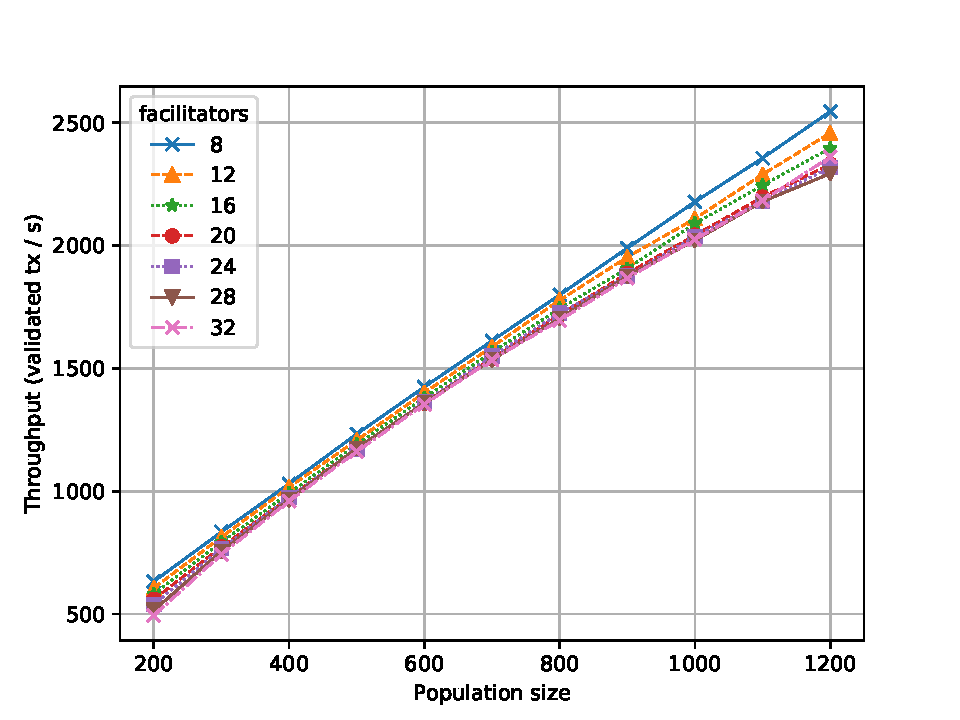
\includegraphics[width=\textwidth]{result-rand-throughput-vs-pop}
  \end{subfigure}
\end{figure}
\section{Evaluation}
\begin{itemize}
  \item How fast is the consensus algorithm? Possibly plot graph of time versus
    the number of nodes.
  \item Does the promoter registration phase add a lot of extra overhead?
  \item What's the rate of transaction such that they can be verified ``on
    time'', i.e. without a growing backlog?
  \item Our global validation rate is somewhat equivalent to the transaction
    rate in other systems. Does the validation rate scale with respect to the
    number of nodes? In theory it should. Plot validation rate vs number of
    nodes, we expect it to be almost linear.
\end{itemize}